\subsection{Other encodings}
\label{sec:data-other}

There are many other lossless data compression schemes described in the literature. Run-length encoding is one such method which encodes substrings consisting of repeated consecutive symbols, known as \textit{runs}, with their repeated symbol and length. First employed in 1967 for transmission of analogue television signals, run-length encoding proves beneficial when there are many runs, especially of long length \cite{rle}. Unfortunately, nanopore signal data does not contain many such runs and would likely encode poorly under this method.

Burrows-Wheeler transform is a data compression preprocessing step used to rearrange data in order to increase its number of runs \cite{bwt}. It is easily reversible, such that the original untransformed data can be obtained from the Burrows-Wheeler transformed data. It has been used to great effect in bioinformatics to compress to basecalled genomic data in the form of FASTQ files \cite{bwt-genomic}.

\subsubsection{Integer compression schemes}
\label{sec:integer-comp}

Bit packing is the process encoding an array of unsigned integers $x_1, x_2, \dots, x_n$
using the smallest number of bits $\hat b$ per integer such that no information is lost.
Consider the integers $1024,12,10,\num{524288}$. The largest $\num{524288}$ can be represented using 20 bits, hence bit packing represents each integer using $\hat b = 20$ bits. Refer to Figure \ref{fig:bitpack} for a visual depiction.
Assume that each integer is typically represented using $b$ bits.
Then, this encoding saves
\[\lfloor \frac{n(b-\hat b)}{8}\rfloor\]
bytes. This equates to a compression ratio of
\begin{align*}
	\text{Compression Ratio} &= \frac{\text{Uncompressed Bytes}}{\text{Compressed Bytes}}\\
	&= \frac{\lceil \frac{nb}{8}\rceil}{\lceil \frac{n\hat b}{8}\rceil}\\
	&\stackrel{n\to\infty}{\longrightarrow}b/\hat b.
\end{align*}
In most programming languages, the integers $1024,12,10,\num{524288}$ would each be represented using 4 bytes or $b=32$ bits.
Hence, on this example the compression ratio would be
\[\frac{\lceil \frac{4 \times 32}{8}\rceil}{\lceil \frac{4 \times 20}{8}\rceil} = 1.6.\]
Compression and decompression using this method can be efficiently computed using scalar processing.
It can be computed even faster by using an alternative bit packing layout and exploiting single-instruction-multiple-data (SIMD) processing  \cite{lemire-simd}.

\begin{figure}
\centering
\begin{tikzpicture}[node distance=0cm,
	start chain=1 going right,
	start chain=2 going right,
	start chain=3 going right,
	start chain=4 going right,
	start chain=5 going right,
	start chain=6 going right,
	start chain=7 going right,
	start chain=8 going right,
	start chain=9 going right,
	start chain=10 going right]
  \tikzstyle{mytape}=[draw]
	\node(a1) [on chain=1,mytape,fill=blue!20] {$0$};
	\node [on chain=1,mytape,fill=blue!20] {$0$};
	\node [on chain=1,mytape,fill=blue!20] {$0$};
	\node [on chain=1,mytape,fill=blue!20] {$0$};
	\node(a2) [on chain=1,mytape,fill=blue!20] {$0$};
	\node [on chain=1,mytape,fill=blue!20] {$0$};
	\node [on chain=1,mytape,fill=blue!20] {$0$};
	\node [on chain=1,mytape,fill=blue!20] {$0$};

	\node [above of=a2,left=-1.65cm,node distance=0.5cm] {$4 \times 20$ bits or $10$ bytes};

	\node(b1) [on chain=2,mytape,fill=blue!20,below of=a1,node distance=0.51cm] {$0$};
	\node [on chain=2,mytape,fill=blue!20] {$0$};
	\node [on chain=2,mytape,fill=blue!20] {$0$};
	\node [on chain=2,mytape,fill=blue!20] {$0$};
	\node [on chain=2,mytape,fill=blue!20] {$0$};
	\node [on chain=2,mytape,fill=blue!20] {$1$};
	\node [on chain=2,mytape,fill=blue!20] {$0$};
	\node [on chain=2,mytape,fill=blue!20] {$0$};

	\node(c1) [on chain=3,mytape,fill=yellow!20,below of=b1,node distance=0.51cm] {$1$};
	\node [on chain=3,mytape,fill=yellow!20] {$1$};
	\node [on chain=3,mytape,fill=yellow!20] {$0$};
	\node [on chain=3,mytape,fill=yellow!20] {$0$};
	\node [on chain=3,mytape,fill=blue!20] {$0$};
	\node [on chain=3,mytape,fill=blue!20] {$0$};
	\node [on chain=3,mytape,fill=blue!20] {$0$};
	\node [on chain=3,mytape,fill=blue!20] {$0$};

	\node(d1) [on chain=4,mytape,fill=yellow!20,below of=c1,node distance=0.51cm] {$0$};
	\node [on chain=4,mytape,fill=yellow!20] {$0$};
	\node [on chain=4,mytape,fill=yellow!20] {$0$};
	\node [on chain=4,mytape,fill=yellow!20] {$0$};
	\node [on chain=4,mytape,fill=yellow!20] {$0$};
	\node [on chain=4,mytape,fill=yellow!20] {$0$};
	\node [on chain=4,mytape,fill=yellow!20] {$0$};
	\node [on chain=4,mytape,fill=yellow!20] {$0$};

	\node(e1) [on chain=5,mytape,fill=yellow!20,below of=d1,node distance=0.51cm] {$0$};
	\node [on chain=5,mytape,fill=yellow!20] {$0$};
	\node [on chain=5,mytape,fill=yellow!20] {$0$};
	\node [on chain=5,mytape,fill=yellow!20] {$0$};
	\node [on chain=5,mytape,fill=yellow!20] {$0$};
	\node [on chain=5,mytape,fill=yellow!20] {$0$};
	\node [on chain=5,mytape,fill=yellow!20] {$0$};
	\node [on chain=5,mytape,fill=yellow!20] {$0$};

	\node(f1) [on chain=6,mytape,fill=green!20,below of=e1,node distance=0.51cm] {$0$};
	\node [on chain=6,mytape,fill=green!20] {$0$};
	\node [on chain=6,mytape,fill=green!20] {$0$};
	\node [on chain=6,mytape,fill=green!20] {$0$};
	\node [on chain=6,mytape,fill=green!20] {$1$};
	\node [on chain=6,mytape,fill=green!20] {$0$};
	\node [on chain=6,mytape,fill=green!20] {$1$};
	\node [on chain=6,mytape,fill=green!20] {$0$};

	\node(g1) [on chain=7,mytape,fill=green!20,below of=f1,node distance=0.51cm] {$0$};
	\node [on chain=7,mytape,fill=green!20] {$0$};
	\node [on chain=7,mytape,fill=green!20] {$0$};
	\node [on chain=7,mytape,fill=green!20] {$0$};
	\node [on chain=7,mytape,fill=green!20] {$0$};
	\node [on chain=7,mytape,fill=green!20] {$0$};
	\node [on chain=7,mytape,fill=green!20] {$0$};
	\node [on chain=7,mytape,fill=green!20] {$0$};

	\node(h1) [on chain=8,mytape,fill=brown!20,below of=g1,node distance=0.51cm] {$0$};
	\node [on chain=8,mytape,fill=brown!20] {$0$};
	\node [on chain=8,mytape,fill=brown!20] {$0$};
	\node [on chain=8,mytape,fill=brown!20] {$0$};
	\node [on chain=8,mytape,fill=green!20] {$0$};
	\node [on chain=8,mytape,fill=green!20] {$0$};
	\node [on chain=8,mytape,fill=green!20] {$0$};
	\node [on chain=8,mytape,fill=green!20] {$0$};

	\node(i1) [on chain=9,mytape,fill=brown!20,below of=h1,node distance=0.51cm] {$0$};
	\node [on chain=9,mytape,fill=brown!20] {$0$};
	\node [on chain=9,mytape,fill=brown!20] {$0$};
	\node [on chain=9,mytape,fill=brown!20] {$0$};
	\node [on chain=9,mytape,fill=brown!20] {$0$};
	\node [on chain=9,mytape,fill=brown!20] {$0$};
	\node [on chain=9,mytape,fill=brown!20] {$0$};
	\node [on chain=9,mytape,fill=brown!20] {$0$};

	\node(j1) [on chain=10,mytape,fill=brown!20,below of=i1,node distance=0.51cm] {$1$};
	\node [on chain=10,mytape,fill=brown!20] {$0$};
	\node [on chain=10,mytape,fill=brown!20] {$0$};
	\node [on chain=10,mytape,fill=brown!20] {$0$};
	\node [on chain=10,mytape,fill=brown!20] {$0$};
	\node [on chain=10,mytape,fill=brown!20] {$0$};
	\node [on chain=10,mytape,fill=brown!20] {$0$};
	\node [on chain=10,mytape,fill=brown!20] {$0$};
\end{tikzpicture}
	\caption[\label{fig:bitpack}The sequence of numbers $1024,12,10,\num{524288}$ in the bit packed format. The data is read from left to right, top to bottom with the most significant bits first.]{\label{fig:bitpack}The sequence of numbers $1024,12,10,\num{524288}$ in the bit packed format. The data is read from left to right, top to bottom with the most significant bits first\protect\footnotemark[1].}
\end{figure}

% TODO move footnotes to the right spot
\footnotetext[1]{Figure \ref{fig:bitpack} is heavily inspired by Figure 1 from \cite{lemire-simd}.}

Stream VByte is a specialised codec for compressing 32-bit unsigned integers \cite{svb}. It stores each integer using a variable number of bytes (1 to 4) depending on its size. Integers in the range $[2^{8(n-1)},2^{8n}-1]$ are represented using $n>0$ bytes. For example, integers in the range $[1,255]$ are losslessly represented using 1 byte. The integer 0 is a special case missing from the above formula which is classically represented using 1 byte. There is however a variation which instead encodes 0 using 0 bytes and integers in the 3 byte range $[2^{16},2^{24}-1]$ with 4 bytes rather than 3. This is advantageous if 0 occurs more often than integers in the 3 byte range. See Table \ref{tab:groupsvb} for a comparison of the classical and 0-based encoding. The number of bytes used for each integer is stored in an array of control bytes which prefaces the actual data. 2-bit words are used to store the number of bytes used for each integer with 00, 01, 10 and 11 corresponding to 1, 2, 3 and 4 bytes respectively (or 0, 1, 2 and 4 bytes in the 0-based variation). See Figures \ref{fig:groupsvb} for an example of how the encodings are structured.

%\begin{tikzpicture}
 	%axis
	\draw (0,0) -- coordinate (x axis mid) (429.4967296,0);
    	\draw (0,0) -- coordinate (y axis mid) (0,4);
    	%ticks
    	\foreach \x in {0,0.0000256,0.0065536,1.6777216,429.4967296}
     		\draw (\x,1pt) -- (\x,-3pt)
			node[anchor=north] {\x};
    	\foreach \y in {0,...,4}
     		\draw (1pt,\y) -- (-3pt,\y)
     			node[anchor=east] {\y};
	%labels
	\node[below=0.8cm] at (x axis mid) {Unsigned 32-bit Integer};
	\node[rotate=90, above=0.8cm] at (y axis mid) {Bytes Used};

	%plots
	\draw (0,1) -- (0.0000256,1);
	\draw (0.0000256,2) -- (0.0065536,2);
	\draw (0.0065536,3) -- (1.6777216,3);
	\draw (1.6777216,4) -- (429.4967296,4);

\end{tikzpicture}

\begin{table}
\centering
    \caption{\label{tab:groupsvb}The number of bytes used and their control codeword for different supported integer ranges in classical 32-bit, 0-based and 16-bit Stream VByte.}
    \begin{tabular}{|l|l|l|l|}%|p{4cm}|p{5.1cm}|}
        \hline
        Stream VByte Method & Integer Range & Number of Bytes Used & Control Codeword\\
        \hline
	    \multirow{4}{3cm}{Classical 32-bit} & $[0,255]$ & 1 & 00\\
	    &$[256,65535]$ & 2 & 01\\
	    &$[65536,16777215]$ & 3 & 10\\
	    &$[16777216,4294967295]$ & 4 & 11\\
        \hline
	    \multirow{4}{4em}{0-based} &$\{0\}$ & 0 & 00\\
	    &$[1,255]$ & 1 & 01\\
	    &$[256,65535]$ & 2 & 10\\
	    &$[65536,4294967295]$ & 4 & 11\\
        \hline
	    \multirow{2}{4em}{16-bit}    &$[0,255]$ & 1 & 0\\
	    &$[256,65535]$ & 2 & 1\\
        \hline
    \end{tabular}
\end{table}

%\subfloat[\label{fig:svb}Compressed classical Stream VByte bytes]{
\centering\begin{tikzpicture}[node distance=0cm,start chain=1 going right,start chain=2 going right] \footnotesize
  \tikzstyle{mytape}=[draw,minimum height=1.4cm]
    \node(Z2)  [on chain=1,mytape,fill=yellow!35] {$00|00|00|01$};

               % \node [above of=Z2,node distance=1cm,fill=blue!10] {\parbox{7cm}{\footnotesize Control bytes are stored in a separate address than the data bytes.}};
    \node(B1)  [on chain=1,mytape,fill=green!35] {$\underbrace{\overbracket{\texttt{0x00}}^{\text{1 byte}}}_{0}$};
    \node(B2)  [on chain=1,mytape,fill=green!35] {$\underbrace{\overbracket{\texttt{0x01}}^{\text{1 byte}}}_{1}$};
    \node(B3)  [on chain=1,mytape,fill=green!35] {$\underbrace{\overbracket{\texttt{0x02}}^{\text{1 byte}}}_{2}$};
    \node(B4)  [on chain=1,mytape,fill=green!35] {$\underbrace{\overbracket{\texttt{0x04}|\texttt{0x00}}^{\text{2 bytes}}}_{\num{1024}}$};


\end{tikzpicture}
%	\caption[An example of $1024,12,10,\num{1048576}, 0,1,2,1024$ compressed with classical and 0-based Stream VByte.]{\label{fig:groupsvb} An example of $1024,12,10,\num{1048576}, 0,1,2,1024$ compressed with classical and 0-based Stream VByte\protect\footnotemark[4].}

\footnotetext[2]{Figures \ref{fig:groupsvb} and \ref{fig:svb-16} are modified versions of Figures 1--3 from \cite{svb}.}

Another variation to this encoding for 16-bit unsigned integers, known as Stream VByte 16, was developed by Oxford Nanopore Technologies in 2022 for compressing nanopore signal data in the POD5 file format \cite{pod5}. It is the same as the classical Stream VByte encoding described above except that each integer is stored using 1 or 2 bytes rather than 1 to 4 bytes. Since there are two different byte lengths, each of the byte lengths is stored using 1 bit; byte lengths 1 and 2 correspond to bit values 0 and 1 respectively. See Table \ref{tab:groupsvb} and Figure \ref{fig:svb-16}. If each integer lies in the range $[0, 2^{16})$ this method saves one bit per integer on average versus classical 32-bit Stream VByte. Due to their similarities, I hypothesise that the compression and decompression speed of Stream VByte 16 is similar if not better than classical Stream VByte. But there is no existing benchmark in the literature which compares both algorithms.

\begin{figure}
\centering
\centering\begin{tikzpicture}[node distance=0cm,start chain=1 going right] \footnotesize
  \tikzstyle{mytape}=[draw,minimum height=1.4cm]
    \node(BIG1)  [on chain=1,mytape,fill=yellow!20] {$\overbracket{1|0|0|1|0|0|0|1}^{\text{control byte}}$};

    \node(A1)  [on chain=1,mytape,fill=green!20,node distance=2cm] {$\underbrace{\overbracket{\texttt{0x04}|\texttt{0x00}}^{\text{2 bytes}}}_{1024}$};
    \node(A2)  [on chain=1,mytape,fill=green!20] {$\underbrace{\overbracket{\texttt{0x0c}}^{\text{1 byte}}}_{12}$};
    \node(A3)  [on chain=1,mytape,fill=green!20] {$\underbrace{\overbracket{\texttt{0x0a}}^{\text{1 byte}}}_{10}$};
	\node(A4)  [on chain=1,mytape,fill=green!20] {$\underbrace{\overbracket{\texttt{0x10}|\texttt{0x00}}^{\text{2 bytes}}}_{\num{4096}}$};
    \node(B1)  [on chain=1,mytape,fill=green!20] {$\underbrace{\overbracket{\texttt{0x00}}^{\text{1 byte}}}_{0}$};
    \node(B2)  [on chain=1,mytape,fill=green!20] {$\underbrace{\overbracket{\texttt{0x01}}^{\text{1 byte}}}_{1}$};
    \node(B3)  [on chain=1,mytape,fill=green!20] {$\underbrace{\overbracket{\texttt{0x02}}^{\text{1 byte}}}_{2}$};
    \node(B4)  [on chain=1,mytape,fill=green!20] {$\underbrace{\overbracket{\texttt{0x04}|\texttt{0x00}}^{\text{2 bytes}}}_{\num{1024}}$};

\end{tikzpicture}
	\caption[\label{fig:svb-16}Compressed 16-bit Stream VByte bytes
	for $1024,12,10,4096, 0,1,2,1024$.]{\label{fig:svb-16}Compressed 16-bit Stream VByte bytes
	for $1024,12,10,4096, 0,1,2,1024$\footnotemark[1].}
\end{figure}


\subsubsection{State-of-the-Art}
\label{sec:state-of-the-art}

This leads us to the current state-of-the-art approach for compressing nanopore signal data which we will name \textit{VBZ16}. VBZ16 is equivalent to VBZ \cite{vbz} but Stream VByte is replaced with Stream VByte 16. VBZ16 consists of the following encodings applied successively:

\begin{enumerate}
\item differential coding,
\item zig-zag encoding,
\item Stream VByte 16 and
\item Zstandard \cite{zstd}.
\end{enumerate}

Differential coding is a bijective function from $\mathbb{R}^n\to\mathbb{R}^n$ classically defined as
\[ (x_1, x_2, \dots, x_n) \mapsto (\delta_1,\delta_2,\dots,\delta_n) = (x_1, x_2 - x_1, x_3-x_2,\dots,x_n-x_{n-1}). \]
That is, the original data is replaced by the differences (or \textit{deltas}) between successive data points.
This transformation is beneficial if the deltas are smaller than the data itself allowing for better compression ratios.
Both the encoding and decoding algorithms for differential coding only require one pass of the data.
However, computation of the \textit{prefix sum} during decompression, defined as
\[ x_1, x_1 + \delta_2, x_1 + \delta_2 + \delta_3, \dots \]
is typically a bottleneck in SIMD optimised applications.
For this reason, there are SIMD-based variations which compute larger deltas, such as $\delta_i = x_i - x_{i-4}$, in exchange for faster decompression times \cite{lemire-simd}.
For nanopore signal data, larger deltas may not actually result in poor compression ratio performance and may be desirable if fast query time is of higher interest.

Zig-zag encoding is another bijection defined as
\begin{align*}
	z&:\mathbb{Z}\to\mathbb{N}_0,\\
	z&(x)=2|x|-\mathbbm{1}_{x<0}(x).
\end{align*}
That is, the negative integers are interleaved with the positive integers such that 0 maps to 0, -1 to 1, 1 to 2, -2 to 3 and so forth.
See Figure \ref{fig:zigzag}.
This encoding allows downstream compression methods to assume all integers are positive and hence ignore the sign-bit from the two's-complement representation.
Whilst also keeping the relative magnitude of numbers the same - numbers close to zero remain close to zero and vice-versa for numbers far from zero.
The zig-zag encoding $z$ of a $b$-bit integer $x$ can be efficiently computed and decoded using standard bitwise operations:
\begin{lstlisting}
z = (x << 1) ^ (x >> (b - 1))
x = (z >>> 1) ^ -(z & 1)
\end{lstlisting}
This technique is used for signed integers in Google Protocol Buffers and is briefly described in their Developer Guide \cite{google-zigzag}.

\begin{figure}
\centering
% Created by tikzDevice version 0.12.3.1 on 2022-09-09 10:58:21
% !TEX encoding = UTF-8 Unicode
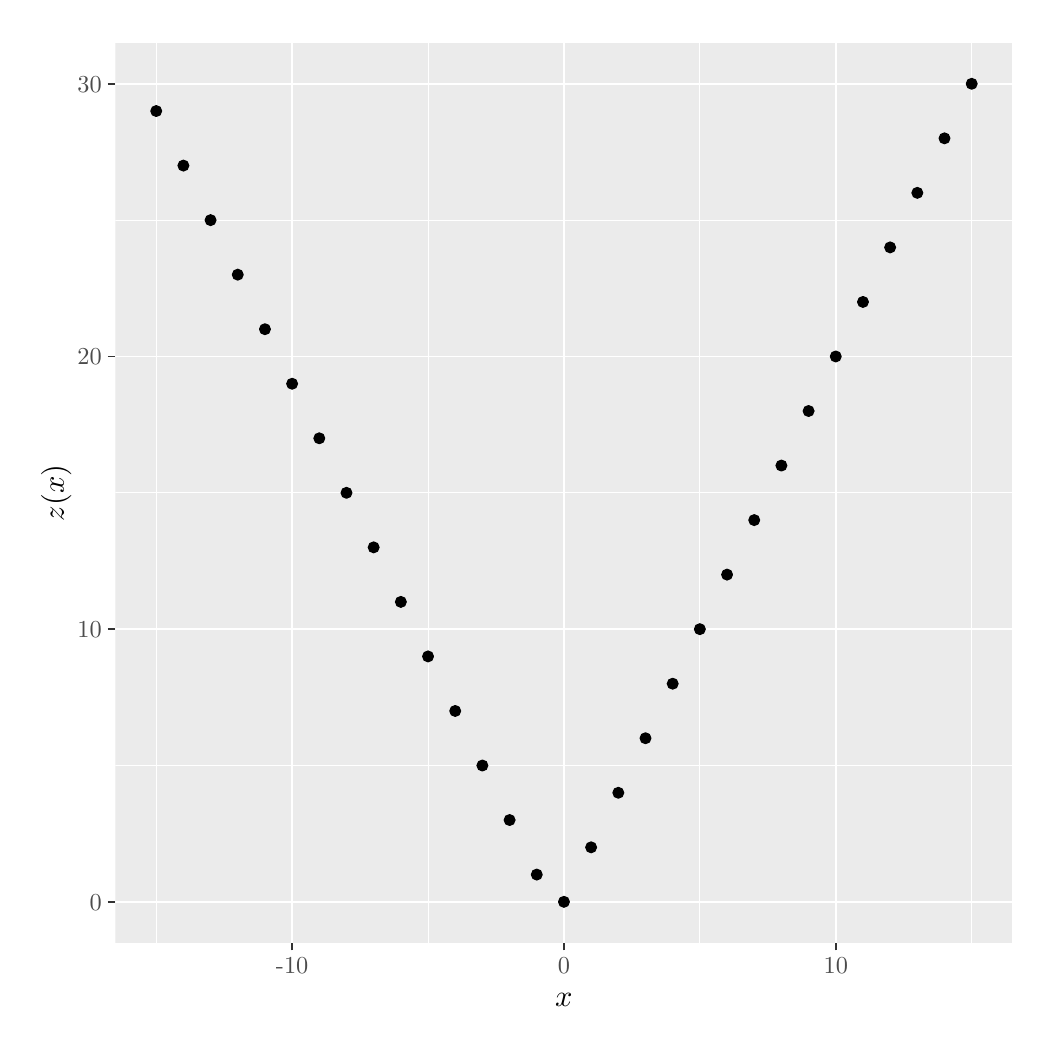
\begin{tikzpicture}[x=1pt,y=1pt]
\definecolor{fillColor}{RGB}{255,255,255}
\path[use as bounding box,fill=fillColor,fill opacity=0.00] (0,0) rectangle (361.35,361.35);
\begin{scope}
\path[clip] (  0.00,  0.00) rectangle (361.35,361.35);
\definecolor{drawColor}{RGB}{255,255,255}
\definecolor{fillColor}{RGB}{255,255,255}

\path[draw=drawColor,line width= 0.6pt,line join=round,line cap=round,fill=fillColor] (  0.00,  0.00) rectangle (361.35,361.35);
\end{scope}
\begin{scope}
\path[clip] ( 31.71, 30.69) rectangle (355.85,355.85);
\definecolor{fillColor}{gray}{0.92}

\path[fill=fillColor] ( 31.71, 30.69) rectangle (355.85,355.85);
\definecolor{drawColor}{RGB}{255,255,255}

\path[draw=drawColor,line width= 0.3pt,line join=round] ( 31.71, 94.73) --
	(355.85, 94.73);

\path[draw=drawColor,line width= 0.3pt,line join=round] ( 31.71,193.27) --
	(355.85,193.27);

\path[draw=drawColor,line width= 0.3pt,line join=round] ( 31.71,291.80) --
	(355.85,291.80);

\path[draw=drawColor,line width= 0.3pt,line join=round] ( 46.45, 30.69) --
	( 46.45,355.85);

\path[draw=drawColor,line width= 0.3pt,line join=round] (144.67, 30.69) --
	(144.67,355.85);

\path[draw=drawColor,line width= 0.3pt,line join=round] (242.89, 30.69) --
	(242.89,355.85);

\path[draw=drawColor,line width= 0.3pt,line join=round] (341.12, 30.69) --
	(341.12,355.85);

\path[draw=drawColor,line width= 0.6pt,line join=round] ( 31.71, 45.47) --
	(355.85, 45.47);

\path[draw=drawColor,line width= 0.6pt,line join=round] ( 31.71,144.00) --
	(355.85,144.00);

\path[draw=drawColor,line width= 0.6pt,line join=round] ( 31.71,242.54) --
	(355.85,242.54);

\path[draw=drawColor,line width= 0.6pt,line join=round] ( 31.71,341.07) --
	(355.85,341.07);

\path[draw=drawColor,line width= 0.6pt,line join=round] ( 95.56, 30.69) --
	( 95.56,355.85);

\path[draw=drawColor,line width= 0.6pt,line join=round] (193.78, 30.69) --
	(193.78,355.85);

\path[draw=drawColor,line width= 0.6pt,line join=round] (292.00, 30.69) --
	(292.00,355.85);
\definecolor{drawColor}{RGB}{0,0,0}
\definecolor{fillColor}{RGB}{0,0,0}

\path[draw=drawColor,line width= 0.4pt,line join=round,line cap=round,fill=fillColor] ( 46.45,331.22) circle (  1.96);

\path[draw=drawColor,line width= 0.4pt,line join=round,line cap=round,fill=fillColor] ( 56.27,311.51) circle (  1.96);

\path[draw=drawColor,line width= 0.4pt,line join=round,line cap=round,fill=fillColor] ( 66.09,291.80) circle (  1.96);

\path[draw=drawColor,line width= 0.4pt,line join=round,line cap=round,fill=fillColor] ( 75.91,272.10) circle (  1.96);

\path[draw=drawColor,line width= 0.4pt,line join=round,line cap=round,fill=fillColor] ( 85.74,252.39) circle (  1.96);

\path[draw=drawColor,line width= 0.4pt,line join=round,line cap=round,fill=fillColor] ( 95.56,232.68) circle (  1.96);

\path[draw=drawColor,line width= 0.4pt,line join=round,line cap=round,fill=fillColor] (105.38,212.97) circle (  1.96);

\path[draw=drawColor,line width= 0.4pt,line join=round,line cap=round,fill=fillColor] (115.20,193.27) circle (  1.96);

\path[draw=drawColor,line width= 0.4pt,line join=round,line cap=round,fill=fillColor] (125.02,173.56) circle (  1.96);

\path[draw=drawColor,line width= 0.4pt,line join=round,line cap=round,fill=fillColor] (134.85,153.85) circle (  1.96);

\path[draw=drawColor,line width= 0.4pt,line join=round,line cap=round,fill=fillColor] (144.67,134.15) circle (  1.96);

\path[draw=drawColor,line width= 0.4pt,line join=round,line cap=round,fill=fillColor] (154.49,114.44) circle (  1.96);

\path[draw=drawColor,line width= 0.4pt,line join=round,line cap=round,fill=fillColor] (164.31, 94.73) circle (  1.96);

\path[draw=drawColor,line width= 0.4pt,line join=round,line cap=round,fill=fillColor] (174.14, 75.03) circle (  1.96);

\path[draw=drawColor,line width= 0.4pt,line join=round,line cap=round,fill=fillColor] (183.96, 55.32) circle (  1.96);

\path[draw=drawColor,line width= 0.4pt,line join=round,line cap=round,fill=fillColor] (193.78, 45.47) circle (  1.96);

\path[draw=drawColor,line width= 0.4pt,line join=round,line cap=round,fill=fillColor] (203.60, 65.17) circle (  1.96);

\path[draw=drawColor,line width= 0.4pt,line join=round,line cap=round,fill=fillColor] (213.43, 84.88) circle (  1.96);

\path[draw=drawColor,line width= 0.4pt,line join=round,line cap=round,fill=fillColor] (223.25,104.59) circle (  1.96);

\path[draw=drawColor,line width= 0.4pt,line join=round,line cap=round,fill=fillColor] (233.07,124.29) circle (  1.96);

\path[draw=drawColor,line width= 0.4pt,line join=round,line cap=round,fill=fillColor] (242.89,144.00) circle (  1.96);

\path[draw=drawColor,line width= 0.4pt,line join=round,line cap=round,fill=fillColor] (252.72,163.71) circle (  1.96);

\path[draw=drawColor,line width= 0.4pt,line join=round,line cap=round,fill=fillColor] (262.54,183.41) circle (  1.96);

\path[draw=drawColor,line width= 0.4pt,line join=round,line cap=round,fill=fillColor] (272.36,203.12) circle (  1.96);

\path[draw=drawColor,line width= 0.4pt,line join=round,line cap=round,fill=fillColor] (282.18,222.83) circle (  1.96);

\path[draw=drawColor,line width= 0.4pt,line join=round,line cap=round,fill=fillColor] (292.00,242.54) circle (  1.96);

\path[draw=drawColor,line width= 0.4pt,line join=round,line cap=round,fill=fillColor] (301.83,262.24) circle (  1.96);

\path[draw=drawColor,line width= 0.4pt,line join=round,line cap=round,fill=fillColor] (311.65,281.95) circle (  1.96);

\path[draw=drawColor,line width= 0.4pt,line join=round,line cap=round,fill=fillColor] (321.47,301.66) circle (  1.96);

\path[draw=drawColor,line width= 0.4pt,line join=round,line cap=round,fill=fillColor] (331.29,321.36) circle (  1.96);

\path[draw=drawColor,line width= 0.4pt,line join=round,line cap=round,fill=fillColor] (341.12,341.07) circle (  1.96);
\end{scope}
\begin{scope}
\path[clip] (  0.00,  0.00) rectangle (361.35,361.35);
\definecolor{drawColor}{gray}{0.30}

\node[text=drawColor,anchor=base east,inner sep=0pt, outer sep=0pt, scale=  0.88] at ( 26.76, 42.44) {0};

\node[text=drawColor,anchor=base east,inner sep=0pt, outer sep=0pt, scale=  0.88] at ( 26.76,140.97) {10};

\node[text=drawColor,anchor=base east,inner sep=0pt, outer sep=0pt, scale=  0.88] at ( 26.76,239.50) {20};

\node[text=drawColor,anchor=base east,inner sep=0pt, outer sep=0pt, scale=  0.88] at ( 26.76,338.04) {30};
\end{scope}
\begin{scope}
\path[clip] (  0.00,  0.00) rectangle (361.35,361.35);
\definecolor{drawColor}{gray}{0.20}

\path[draw=drawColor,line width= 0.6pt,line join=round] ( 28.96, 45.47) --
	( 31.71, 45.47);

\path[draw=drawColor,line width= 0.6pt,line join=round] ( 28.96,144.00) --
	( 31.71,144.00);

\path[draw=drawColor,line width= 0.6pt,line join=round] ( 28.96,242.54) --
	( 31.71,242.54);

\path[draw=drawColor,line width= 0.6pt,line join=round] ( 28.96,341.07) --
	( 31.71,341.07);
\end{scope}
\begin{scope}
\path[clip] (  0.00,  0.00) rectangle (361.35,361.35);
\definecolor{drawColor}{gray}{0.20}

\path[draw=drawColor,line width= 0.6pt,line join=round] ( 95.56, 27.94) --
	( 95.56, 30.69);

\path[draw=drawColor,line width= 0.6pt,line join=round] (193.78, 27.94) --
	(193.78, 30.69);

\path[draw=drawColor,line width= 0.6pt,line join=round] (292.00, 27.94) --
	(292.00, 30.69);
\end{scope}
\begin{scope}
\path[clip] (  0.00,  0.00) rectangle (361.35,361.35);
\definecolor{drawColor}{gray}{0.30}

\node[text=drawColor,anchor=base,inner sep=0pt, outer sep=0pt, scale=  0.88] at ( 95.56, 19.68) {-10};

\node[text=drawColor,anchor=base,inner sep=0pt, outer sep=0pt, scale=  0.88] at (193.78, 19.68) {0};

\node[text=drawColor,anchor=base,inner sep=0pt, outer sep=0pt, scale=  0.88] at (292.00, 19.68) {10};
\end{scope}
\begin{scope}
\path[clip] (  0.00,  0.00) rectangle (361.35,361.35);
\definecolor{drawColor}{RGB}{0,0,0}

\node[text=drawColor,anchor=base,inner sep=0pt, outer sep=0pt, scale=  1.10] at (193.78,  7.64) {$x$};
\end{scope}
\begin{scope}
\path[clip] (  0.00,  0.00) rectangle (361.35,361.35);
\definecolor{drawColor}{RGB}{0,0,0}

\node[text=drawColor,rotate= 90.00,anchor=base,inner sep=0pt, outer sep=0pt, scale=  1.10] at ( 13.08,193.27) {$z(x)$};
\end{scope}
\end{tikzpicture}

\caption{\label{fig:zigzag}The zig-zag encoding applied to integers -15 to 15. As we can see, it is similar to the absolute value function but is doubled and shifted on the negative $x$-axis to ensure injectivity.}
\end{figure}


This requires at least four passes over the input data depending on how many passes Zstandard performs.
